\section{IR-analyse af stofferne paracetamol, ibuprofen og R-limonen}
Vi vil i dette afsnit se nærmere på hvordan man i praksis bestemmer hvilket stof et bestemt IR-spektrogram hører til. Der vil ses på de tre stoffer: paracetamol, som er et udbredt smertestillende middel, ibuprofen, der også er smertestillende og til sidst stoffet R-limonen, som er en farveløs væske der ved stuetemperatur dufter kraftigt af appelsin (FODNOTE WIKI). Vi har tre forskellige stoffer vi skal tildele til tre forskellige IR-spektre. Man kan indledningsvist se på molekylernes opbygning og gøre det klart for sig selv, hvilke steder man forventer at se absorption. 
\\

Der kigges da på de funktionelle grupper som de tre stoffer indeholder

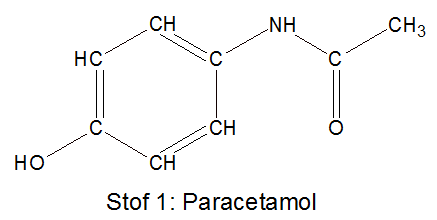
\includegraphics[scale=0.5]{Billeder/paracetamol}
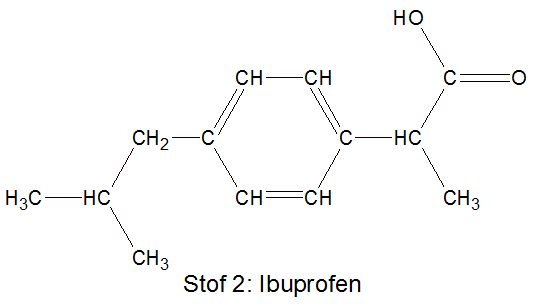
\includegraphics[scale=0.5]{Billeder/ibuprofen}
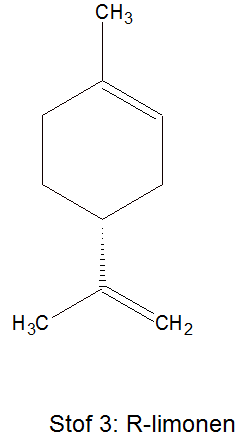
\includegraphics[scale=0.5]{Billeder/Rlimonen}
\vspace{0.8cm}
\begin{enumerate}
\item[\textbf{Stof 1}] 
Stof 1 er paracetamol. De karakteristiske bølgetal for funktionelle grupper vi har tænkt at at kigge efter, når vi skal slå op i vores tabel for bølgetal er følgende: 
\begin{itemize}
\item OH-Ar Fenol, da vi har en alkoholgruppe, som sidder på en aromatisk ring. (\={v}= 3550-3200)

\item N-H: sekundær amid, da vi har en carbonylgruppe, som er bundet til et nitrogenatom, der kun er bundet til 1 hydrogenatom. (\={v}= 3400-3500 og ~1650)

\item CH: $sp^2$-stræk fra den aromatiske ring (\={v}=3010-3100 )

\item C=O: Amidgruppen giver udslag i området (\={v}= 1600-1700)

\item C-H $sp^3$-stræk i området (\={v}= 2810-2960)
\end{itemize}

\item[\textbf{Stof 2}]
Stof 2 er Ibuprofen. Vi er igen interesserede i de karakteristiske bølgetal for de funktionelle grupper som stoffet indeholder. Vi skriver dem op i tabellen nedenfor. 

\begin{itemize}
\item C-H: $sp^3$-stræk i området (\={v}= 2810-2960)

\item CH: $sp^2$-stræk i intervallet (\={v}= 3010-3100) for den aromatiske ring. 

\item C=O: Carboxylsyregruppen i ibuprofen giver udslag i området om (\={v}= 1695)

\item O-H: Hydroxylgruppen i ibuprofen giver udslag i området (\={v}= 3500-2500) og er et meget bredt bånd. 
\end{itemize}
\item[\textbf{Stof 3}]
De karakteristiske bølgetal for de funktionelle grupper i R-limonen skrives op

\item H-C=: Bindingen mellem hydrogenatomet og carbonatomet, der sidder i en dobbeltbinding med et andet carbonatom giver udslag i området (\={v}=  3010-3100)

\item C-H $sp^3$: giver udslag i området (\={v}= 2810-2960) 

\item C=C $sp^2$: Giver udslag i området (\={v}= 1600-1700) 
\end{enumerate}

De tre stoffer skal nu knyttes til hver deres IR-spektrogram ( SE BILAG MANGLER). For at overskueliggøre denne process, tager vi udgangspunkt i forskellene på de funktionelle grupper som de tre stoffer indeholder. R-limonen indeholder for eksempel ikke nogen hydroxylgruppe og vil ikke have det kendetegnende brede \emph{tungebånd} i området omkring (\={v} $\approx$ 3000). Hvis vi kigger på bilagene med IR-spektrogrammerne kan vi se, at dette udelukker både bilag 1 og 2. Vi kan altså næsten øjeblikkeligt slutte, at stoffet R-limonen hører til IR-spektrogrammet på bilag 3. Vi vælger dog at undersøge det lidt nærmere for en sikkerheds skyld. 
\\

Hvis bilag 3 skulle være IR-spektrogrammet af R-limonen skulle vi se absorbtionsbånd for de funktionelle grupper der er i R-limonen. Dette var  et et udslag i området (\={v}= 1600-1700) - Dette kan vi bekræfte også er der på bilag 3, et udslag i området (\={v}= 2810-2960) - dette er også tilstedeværende på vores spektrogram, og et udslag ved (\={v}= 3010-3100) som formegentligt er blevet forskudt lidt mod højre og flyder ud $sp^2$-båndet.
\\

Med alt taget i betragtning virker bilag 3 til at være et godt bud på at være et IR-spektrogram af R-limonen.

